%\pdfminorversion=4
\documentclass[9pt]{beamer}
\usetheme{default}
\useinnertheme[shadow]{rounded}

%\useoutertheme[left,hideothersubsections]{IGNsidebar}
\useoutertheme[left,hideothersubsections]{IGNsidebar}




%/usr/share/texmf/tex/latex/beamer/themes/font/beamerfontthemedefault.sty
%/usr/share/texmf/tex/latex/beamer/themes/font/beamerfontthemeprofessionalfonts.sty
%/usr/share/texmf/tex/latex/beamer/themes/font/beamerfontthemeserif.sty
%/usr/share/texmf/tex/latex/beamer/themes/font/beamerfontthemestructurebold.sty
%/usr/share/texmf/tex/latex/beamer/themes/font/beamerfontthemestructureitalicserif.sty
%/usr/share/texmf/tex/latex/beamer/themes/font/beamerfontthemestructuresmallcapsserif.sty
\usefonttheme{structurebold}

% %%%%%%%%%%%%%%%%%%%%%%%%%%%%%%%%%%%%%%%%%%%%%%%%%%%  packages----------------------
\RequirePackage{tikz}
\usetikzlibrary{arrows}
\usepackage[utf8]{inputenc}
\RequirePackage{tikz}

\usetikzlibrary{calc}

%\usepackage{gnuplottex}
\usepackage{movie15}



% - Objets flottants
\usepackage{graphicx}
\usepackage{booktabs}
%\usepackage{multimedia}
% - Liens et hyperliens
\usepackage{hyperref}
\usepackage{animate}
% - Maths et unit�s
%\usepackage[amssymb]{SIunits}
%\usepackage{amssymb}
\usepackage{amsmath}
\usepackage{lastpage}

\usepackage{graphicx}
\usepackage[squaren,Gray]{SIunits}
% - Liens et hyperliens
\usepackage{ragged2e}
\justifying
%\usepackage[]{algorithm2e}
\usepackage{algorithm2e}
\usepackage{multirow}
%Tabulars with adjustable-width columns.
\usepackage{array}

\renewcommand{\textbf}[1]{\begingroup\bfseries\mathversion{bold}#1\endgroup}

\definecolor{IGNVert}{RGB}{148, 192,  22}
\definecolor{IGNGris}{RGB}{112, 119, 122}

\definecolor{IGNRouge}{RGB}{255, 100, 100}
\definecolor{IGNOrange}{RGB}{230, 126, 48}


\definecolor{colortype1}{RGB}{255,127,0}
\definecolor{colortype2}{RGB}{255,0,0}
\definecolor{colortype3}{RGB}{255,0,255}
\definecolor{colortype4}{RGB}{255,255,0}
\definecolor{colortype5}{RGB}{0,255,0}
\definecolor{colortype6}{RGB}{0,100,0}
\definecolor{colortype7}{RGB}{0,255,255}
\definecolor{colortype8}{RGB}{0,0,255}
\definecolor{colortype9}{RGB}{0,0,100}

\definecolor{minuit}{RGB}{0,0,128}
\definecolor{banane}{RGB}{255,255,100}
\definecolor{fougere}{RGB}{64,128,0}
\definecolor{citronvert}{RGB}{128,255,0}
\definecolor{aqua}{RGB}{0,128,255}

\definecolor{darkblue}{rgb}{0.0, 0.0, 0.55}
\definecolor{darkmagenta}{rgb}{0.55, 0.0, 0.55}
\definecolor{darkgreen}{rgb}{0.0, 0.2, 0.13}
\definecolor{darkred}{rgb}{0.55, 0.0, 0.0}

\definecolor{cafafaf}{RGB}{175,175,175}
\definecolor{c646464}{RGB}{100,100,100}
\definecolor{c007d00}{RGB}{0,125,0}

\newcommand\imp[1]{\textcolor{IGNVert}{\textbf{#1}}}


%PUCES
\setbeamercolor{item projected}{bg=IGNGris!70}

%%%%%%%%%%%%%%%%%%%%%%%%%%%%%%%%%%%%%%%%%%%%%%%%%%% COLOR
\setbeamercolor*{normal text}{fg=IGNGris}

\setbeamercolor{title}{fg=IGNGris}
\setbeamercolor{subtitle}{fg=IGNVert}
\setbeamercolor{item}{fg=IGNVert} 

\setbeamercolor{caption name}{ fg=IGNGris}

\setbeamercolor{author in head/foot}{ fg=IGNGris}
\setbeamercolor{institute in head/foot}{fg=IGNGris}
\setbeamercolor{title in head/foot}{ fg=IGNGris}
\setbeamercolor{date in head/foot}{ fg=IGNGris}
\setbeamercolor{page in head/foot}{ fg=IGNGris}
\setbeamercolor{section in toc}{ fg=IGNGris}
\setbeamercolor{subsection in toc}{ fg=IGNGris}

\setbeamercolor*{block title alerted}{bg=IGNRouge!70}
\setbeamercolor*{block body alerted}{bg=IGNRouge!20}

\setbeamercolor*{block title example}{bg=IGNGris!50}
\setbeamercolor*{block body example}{bg=IGNGris!20}

\setbeamercolor*{block title}{bg=IGNVert!70}
\setbeamercolor*{block body}{bg=IGNVert!20}

%%%%%%%%%%%%%%%%%%%%%%%%%%%%%%%%%%%%%%%%%%%%%%%%%%% NAVIGATION SYMBOLS
\setbeamertemplate{navigation symbols}{} 
%%%%%%%%%%%%%%%%%%%%%%%%%%%%%%%%%%%%%%%%%%%%%%%%%%% SIDE BAR
\setbeamersize{sidebar width left=1.2cm}
\setbeamercolor{section in sidebar}{fg=IGNGris}
\setbeamercolor{subsection in sidebar}{fg=IGNGris}

\setbeamercolor{section in sidebar shaded}{fg=IGNVert}
\setbeamercolor{subsection in sidebar shaded}{fg=IGNVert}

%tikz
\usepackage{tikz}
\usetikzlibrary{shapes.multipart}
\usetikzlibrary{automata}
\usetikzlibrary{arrows,shapes}
\usetikzlibrary{trees,positioning}
\usetikzlibrary{chains,matrix,scopes,decorations.pathmorphing,shadows}
\usetikzlibrary{plotmarks}
\usetikzlibrary{decorations.markings}
\usetikzlibrary{patterns}
\definecolor{cafafaf}{RGB}{175,175,175}
\definecolor{c646464}{RGB}{100,100,100}
\definecolor{c007d00}{RGB}{0,125,0}
\defbeamertemplate*{sidebar}{SSB}{}

\usepackage{pifont}								% checkmark and crossmark
\newcommand{\cmark}{\ding{51}}
\newcommand{\xmark}{\ding{55}}
\newcommand{\IGNArrow}{\textcolor{IGNVert}{\ding{230}}}


%%%%%%%%%%%%%%%%%%%%%%%%%%%%%%%%%%%%%%%%%%%%%%%%%%% HEAD LINE
\defbeamertemplate*{frametitle}{}{
\vspace{+0,3cm}

    \textcolor{IGNGris}{ \textbf{\insertframetitle}}
    
\vspace{-0,3cm}    
     
  \begin{tikzpicture}
  \draw[very thick,color=IGNVert] (0,1)--(\paperwidth- 2.24,1);
  \end{tikzpicture} 
  
  
}
%%%%%%%%%%%%%%%%%%%%%%%%%%%%%%%%%%%%%%%%%%%%%%%%%%% HEAD LINE
%\defbeamertemplate*{headline}{AH}{
%}

\defbeamertemplate*{headline}{}{}
%%%%%%%%%%%%%%%%%%%%%%%%%%%%%%%%%%%%%%%%%%%%%%%%%%% BACKGROUND

%%%%%%%%%%%%%%%%%%%%%%%%%%%%%%%%%%%%%%%%%%%%%%%%%%% FOOT LINE
\defbeamertemplate*{footline}{}
{
\leavevmode%
  \begin{tikzpicture}
  \draw (0,0) node  {};
  \draw (0.5,0) node[right]  { \textcolor{IGNGris}{\insertshorttitle}};
  %\draw (5,0) node[right]  { \textcolor{IGNVert}{$\blacksquare$} \textcolor{IGNGris}{\insertshortdate{} } };
  \draw (8.5,0) node  { \textcolor{IGNVert}{$\blacksquare$} \textcolor{IGNGris}{\insertframenumber{} / \inserttotalframenumber\hspace*{2ex} }};
 \draw (9.75,0) node  { \textcolor{IGNGris}{ \insertshortinstitute }};
  \draw (11.7,0) node[right] { 
\includegraphics[height=0.25cm]{ressources/template/logos/ENSG-simplifie2} };
  \end{tikzpicture} 

}%


%%%%%%%%%%%%%%%%%%%%%%%%%%%%%%%%%%%%%%%%%%%%%%%%%%% AT BEGIN SECTION


\AtBeginSection[]
{ 
\setbeamercolor{section in sidebar}{fg=white }
\setbeamercolor{subsection in sidebar}{fg=white }

\setbeamercolor{section in sidebar shaded}{fg=white }
\setbeamercolor{subsection in sidebar shaded}{fg=white }



\begin{frame}{
  \begin{tikzpicture}[scale=0.503]
  \draw[color=IGNGris,fill=IGNGris]  (0,0) rectangle (23,9);
  \draw (1,1) node [right,text width=10cm,text justified]  {  \textcolor{white}{\insertsection}};
  \end{tikzpicture}
}
\end{frame} 


\setbeamercolor{section in sidebar}{fg=IGNGris}
\setbeamercolor{subsection in sidebar}{fg=IGNGris}

\setbeamercolor{section in sidebar shaded}{fg=IGNVert}
\setbeamercolor{subsection in sidebar shaded}{fg=IGNVert}

\addtocounter{framenumber}{-1}

}



\title{Estimation de la densité dans l'espace urbain piéton}

\subtitle{M2-IGAST / Projet d'Analyse Spatiale}
\date{}

\author{Paul Chapron}
\institute[]{
Univ. Gustave Eiffel, LASTIG, IGN-ENSG, Saint-Mandé, France.  \\
}
\date{\today}

\usepackage[french]{babel}
\usepackage{datetime}  
\usepackage[T1]{fontenc}

\usepackage{hyperref}
\hypersetup{
    unicode=false,             % non-Latin characters in Acrobat’s bookmarks
    pdftoolbar=true,           % show Acrobat’s toolbar?
    pdfmenubar=true,           % show Acrobat’s menu?
    pdffitwindow=false,        % window fit to page when opened
    pdfstartview={FitH},       % fits the width of the page to the window
    pdftitle={Sujet Projet AS IGAST: KDE \& pathfinding }, % title
    pdfnewwindow=true,         % links in new PDF window
    colorlinks=true,           % false: boxed links; true: colored links
    linkcolor=IGNVert,             % color of internal links (change box color with linkbordercolor)
    citecolor=green,           % color of links to bibliography
    filecolor=magenta,         % color of file links
    urlcolor=teal   % color of external links
}


% Backup frames
%\setcounter{framenumber}{38}

\begin{document}

%%%%%%%%%%%%%%%%%%%%%%%%%%%%%%%%%%%%%%%%%%%%%%%%%%%%%%%%%%%%%%%%%%%%%%%%%%%%%%%%%%%%%%%%%%%%%%%%%%%%%%%%%
% FRAME DE COUVERTURE
% MODELE 1

\begin{frame}[plain,c]
\begin{columns}
\begin{column}{8cm}
\begin{center}
\vspace{2cm}
\titlepage
\end{center}
\end{column}
\begin{column}{1cm}
\end{column}
\end{columns}

\end{frame}




%%%%%%%%%%%%%%%%%%%%%%%%%%%%%%%%%%%%%%%%%%%%%%%%%%%%%%%%%%%%%%%%%%%%%%%%%%%%%%%%%%%%%%%%%%%%%%%%%%%%%%%%%
% DEBUT DE LA PRESENTATION
% BACKGROUND POUR AVOIR LE HAUT DE PAGE QUI VA BIEN
\usebackgroundtemplate{
    \begin{tikzpicture}[scale=0.503]
    \filldraw[color=IGNGris] (0,0) rectangle(2.62,0.54);
    \filldraw[color=IGNGris] (4.77,0) rectangle(2.62+4.77,0.54);
    
    \filldraw[color=IGNVert] (9.50+0.27,0) -- (9.50,0.54)-- (9.50+7.41-0.27,0.54)-- (9.50+7.41,0)--cycle;
    
    \filldraw[color=IGNGris] (19.50,0) rectangle(2.62+19.50,0.54);
    \filldraw[color=IGNGris] (23.11,0.54)--(23.11+0.54,0)--(2.3+23.11,0)--(2.3+23.11,0.54)--cycle;;
    \end{tikzpicture}   
}
\setbeamercolor{alerted text}{fg=IGNVert}


%%%%%%%%%%%%%%%%%%%%%%%%%%%%%%%%%%%%%%%%%%%%%%%%%%%%%%%%%%%%%%%%%%%%%%%%%%%%%%%%%%%%%%%%%%%%%%%%%%%%%%%%%
% PLAN
\setbeamercolor{section in sidebar}{fg=white } %LIGNE NECESSAIRE POUR EFFACER LE PLAN DE LA SIDEBAR (PAS MIEUX)
\setbeamercolor{subsection in sidebar}{fg=white }%LIGNE NECESSAIRE POUR EFFACER LE PLAN DE LA SIDEBAR (PAS MIEUX)
\setbeamercolor{section in sidebar shaded}{fg=white }%LIGNE NECESSAIRE POUR EFFACER LE PLAN DE LA SIDEBAR (PAS MIEUX)
\setbeamercolor{subsection in sidebar shaded}{fg=white }%LIGNE NECESSAIRE POUR EFFACER LE PLAN DE LA SIDEBAR (PAS MIEUX)
%\begin{frame}
  %\begin{columns}[T]
  %\begin{column}{5cm}
  %\tableofcontents[sections={1-2}, hideallsubsections]
  %\end{column}
  %\begin{column}{5cm}
  %\tableofcontents[sections={3-4}, hideallsubsections]
  %\end{column}
  %\end{columns}
%\end{frame}
\setbeamercolor{section in sidebar}{fg=IGNGris}%LIGNE NECESSAIRE POUR AFFICHER LE PLAN DE LA SIDEBAR (PAS MIEUX)
\setbeamercolor{subsection in sidebar}{fg=IGNGris}%LIGNE NECESSAIRE POUR AFFICHER LE PLAN DE LA SIDEBAR (PAS MIEUX)
\setbeamercolor{section in sidebar shaded}{fg=IGNVert}%LIGNE NECESSAIRE POUR AFFICHER LE PLAN DE LA SIDEBAR (PAS MIEUX)
\setbeamercolor{subsection in sidebar shaded}{fg=IGNVert}%LIGNE NECESSAIRE POUR AFFICHER LE PLAN DE LA SIDEBAR (PAS MIEUX)





%%%%%%%%%%%%%%%%%%%%%%%%%%%%%%%%%%%%%%%%%%%%%%%%%%%%%%%%%%%%%%%%%%%%%%%%%%%%%%%%%%%%%%%%%%%%%%%%%%%%%%%%%
%%% PRESENTATION BEAMER CLASSIQUE

%%%%%%%%%%%%%%%%%%%%%%%%%%%%%%%%%%%%% Organisation %%%%%%%%%%%%%%%%%%%%%%%%%%%%%%%%%%%%%%%%%%%%%%%%%%%%%%%%%



\begin{frame}{L'estimation de densité 2D}

Kernel Density Estimate (KDE): méthode statistique qui estime la densité de probabilité d'une variable aléatoire \alert{en tout point du support } à l'aide d'un \textit{noyau} (souvent gaussien)\\
\begin{center}
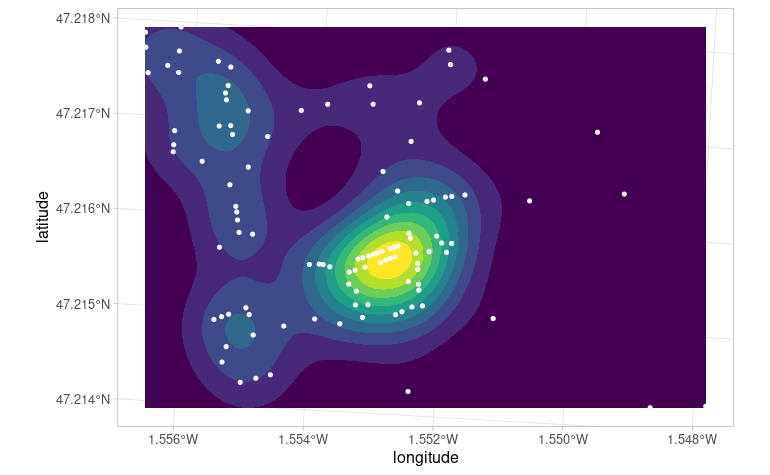
\includegraphics[height=0.3\textwidth]{ressources/images/KDE_raster.png} 
\end{center}


Notion de \alert{distance} :  noyau gaussien $\rightarrow$ contribution d'une observation fonction inverse de sa distance  \\


\vspace{0.5cm}



\begin{scriptsize}
2 caractéristiques à noter  

\begin{itemize} 
  \item Le calcul peut être fait en tout point 
  \item La distance "classique" est euclidienne
\end{itemize}




\end{scriptsize}
\end{frame}




\begin{frame}{Problématique: Densité(s) dans l'espace piéton urbain }

Hypothèse : la densité de \alert{piétons} en centre ville se modélise comme une combinaison de densité de \alert{points d'intérêts} (POI)\\
\begin{scriptsize}
  e.g. boutiques, cinémas, arrêts TPC, restauration, musées, lieux de culte, etc.
\end{scriptsize}
\vspace{0.5cm}

Constats : 
\begin{itemize}
  \item inutile de calculer une densité là où on ne peut pas marcher 
  \item la distance euclidienne n'est pas adaptée à la marche en centre ville
\end{itemize}
\vspace{0.5cm}

Objectif : Calculer une densité 2D \alert{plausible} pour un piéton i.e.

\begin{itemize}
  \item uniquement dans les zones «marchables» $\rightarrow$ \alert{à construire}
  \item avec une distance «à pied» $\rightarrow$  \alert{pathfinding}
\end{itemize}
\vspace{0.5cm}
pour différentes couches de points d'intérêt
\end{frame}


\begin{frame}{Zone «marchable» à Nantes}
\begin{center}
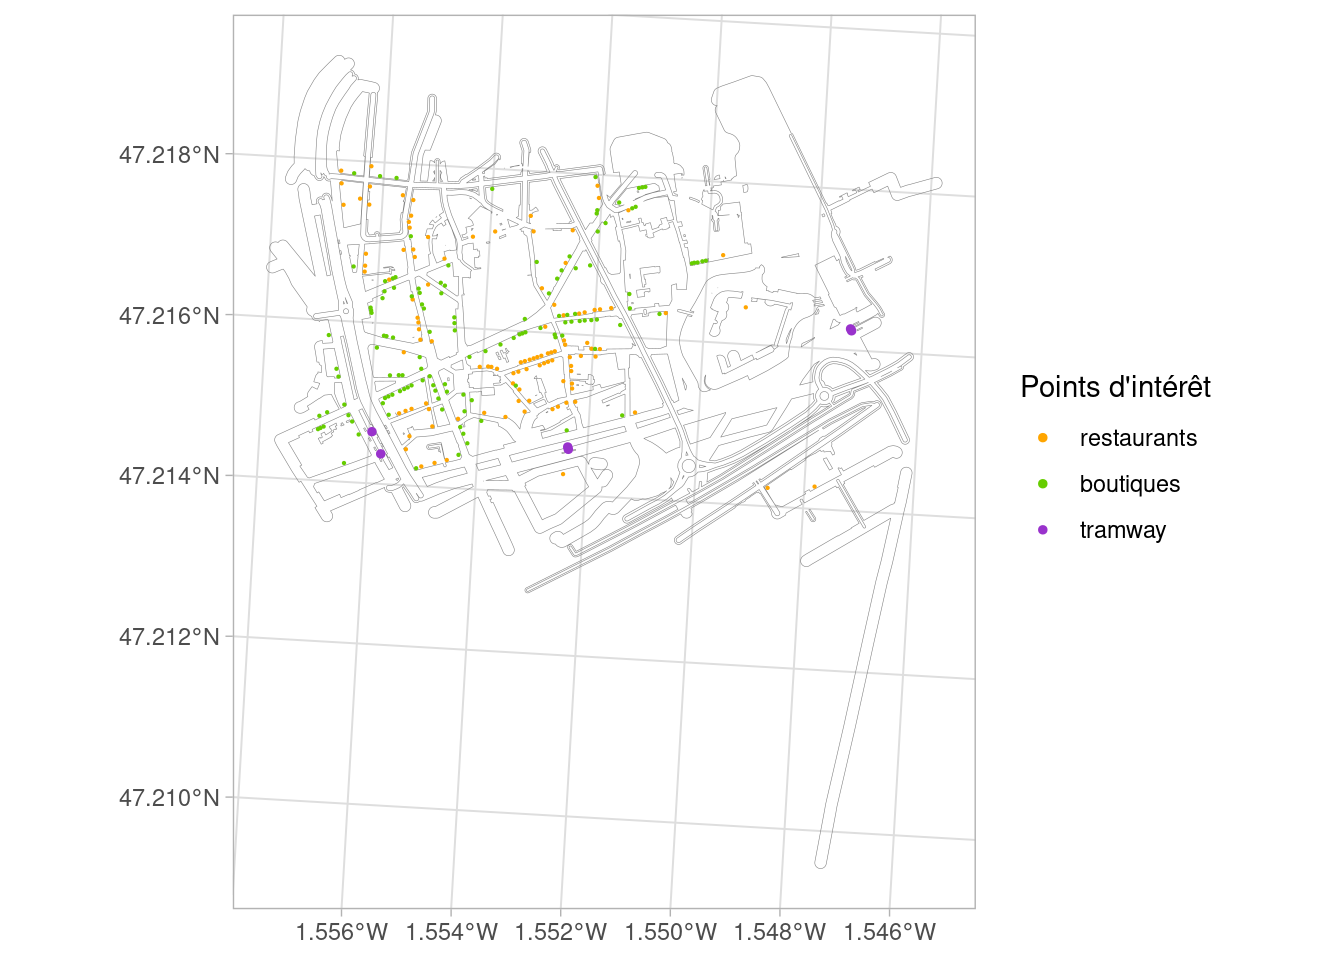
\includegraphics[width=\textwidth]{ressources/images/zone_marchable.png} 
\end{center}
\end{frame}



\begin{frame}{Outils libres et données ouvertes}


\textbf{Données :} Jeu de données de test fourni, extension avec extraction d'OSM et/ou IGN \\ 

\vspace{0.5cm}

 \textbf{Outils :} R (obligatoire), IDE, librairies recommandées :



\begin{center}

\includegraphics[height=0.1\textwidth]{ressources/images/rlogo.jpg} 

\includegraphics[height=0.1\textwidth]{ressources/images/rstudio.png}  

\includegraphics[height=0.1\textwidth]{ressources/images/sf_logo.png} 

\includegraphics[height=0.1\textwidth]{ressources/images/logo_osmdata.png} 
\end{center}

\vspace{0.9cm}

\begin{scriptsize}
\begin{itemize}
\item R \url{https://cran.rstudio.com/}
\item Rstudio \url{https://posit.co/download/rstudio-desktop/}
\item package sf \url{https://r-spatial.github.io/sf/}
\item tuto R  + sf en français \url{https://hackmd.io/@hOaFaD2DS4WcOzNXU6j7vg/HJThOyWvU}
\item librairie R d'import OSM  \url{https://github.com/ropensci/osmdata}
\end{itemize}
\end{scriptsize}

\end{frame}

%
%

\begin{frame}{Livrables attendus }

\begin{itemize}
\item Code versionné sur \url{https://github.com/chapinux/KDE_pathfinding}
\item Documentation succincte
\item Rapport
\item Diaporama de soutenance
\end{itemize}



\end{frame}






%%%%%%%%%%%%%%%%%%%%%%%%%%%%%%%%%%%%% Révision raster sources de données et résolutions %%%%%%%%%%%%%%%%%%%%%%%%%%%%%%%%%












%%%%%%%%%%%%%%%%%%%%%%%%%%%%%%%%%%%%%%%%%%%%%%%%%%%%%%%%%%%%%%%%%%%%%%%%%%%%%%%%%%%%%%%%%%%%%%%%%%%%%%%%%
%%% BIBLIOGRAPHIE ET FIN

%\begin{frame}{Bibliographie}
%\begin{figure}[!h]
%\begin{center}
% \begin{tabular}{cccc}
%   \toprule
%   \includegraphics[height=7cm]{images/bookmassonnet}   & \includegraphics[height=7cm]{images/bookmaitreRSO} \\
%     \bottomrule
% \end{tabular}\\
%\cite{massonnet2008}, \cite{maitre2001}
%\end{center}
%\end{figure}
%\end{frame}




% DEBUT DE LA PRESENTATION
% BACKGROUND POUR AVOIR LE HAUT DE PAGE QUI VA BIEN
\usebackgroundtemplate{
    \begin{tikzpicture}[scale=0.503]
    \filldraw[color=IGNGris] (0,0) rectangle(2.62,0.54);
    \filldraw[color=IGNGris] (4.77,0) rectangle(2.62+4.77,0.54);
    
    \filldraw[color=IGNVert] (9.50+0.27,0) -- (9.50,0.54)-- (9.50+7.41-0.27,0.54)-- (9.50+7.41,0)--cycle;
    
    \filldraw[color=IGNGris] (19.50,0) rectangle(2.62+19.50,0.54);
    \filldraw[color=IGNGris] (23.11,0.54)--(23.11+0.54,0)--(2.3+23.11,0)--(2.3+23.11,0.54)--cycle;;
    \end{tikzpicture}   
}

%\begin{frame}[allowframebreaks]{Bibliographie}
%\nocite{} 
%\bibliographystyle{apalike} 
%\bibliography{ressources/biblio/biblio-cours} % .bib file
% \end{frame}  

\end{document}

